\begin{titlepage}
%----------------------------------------------------------------------------------------
%	TITLE PAGE
%----------------------------------------------------------------------------------------

\begingroup
\thispagestyle{empty}
\AddToShipoutPicture*{\put(0,0){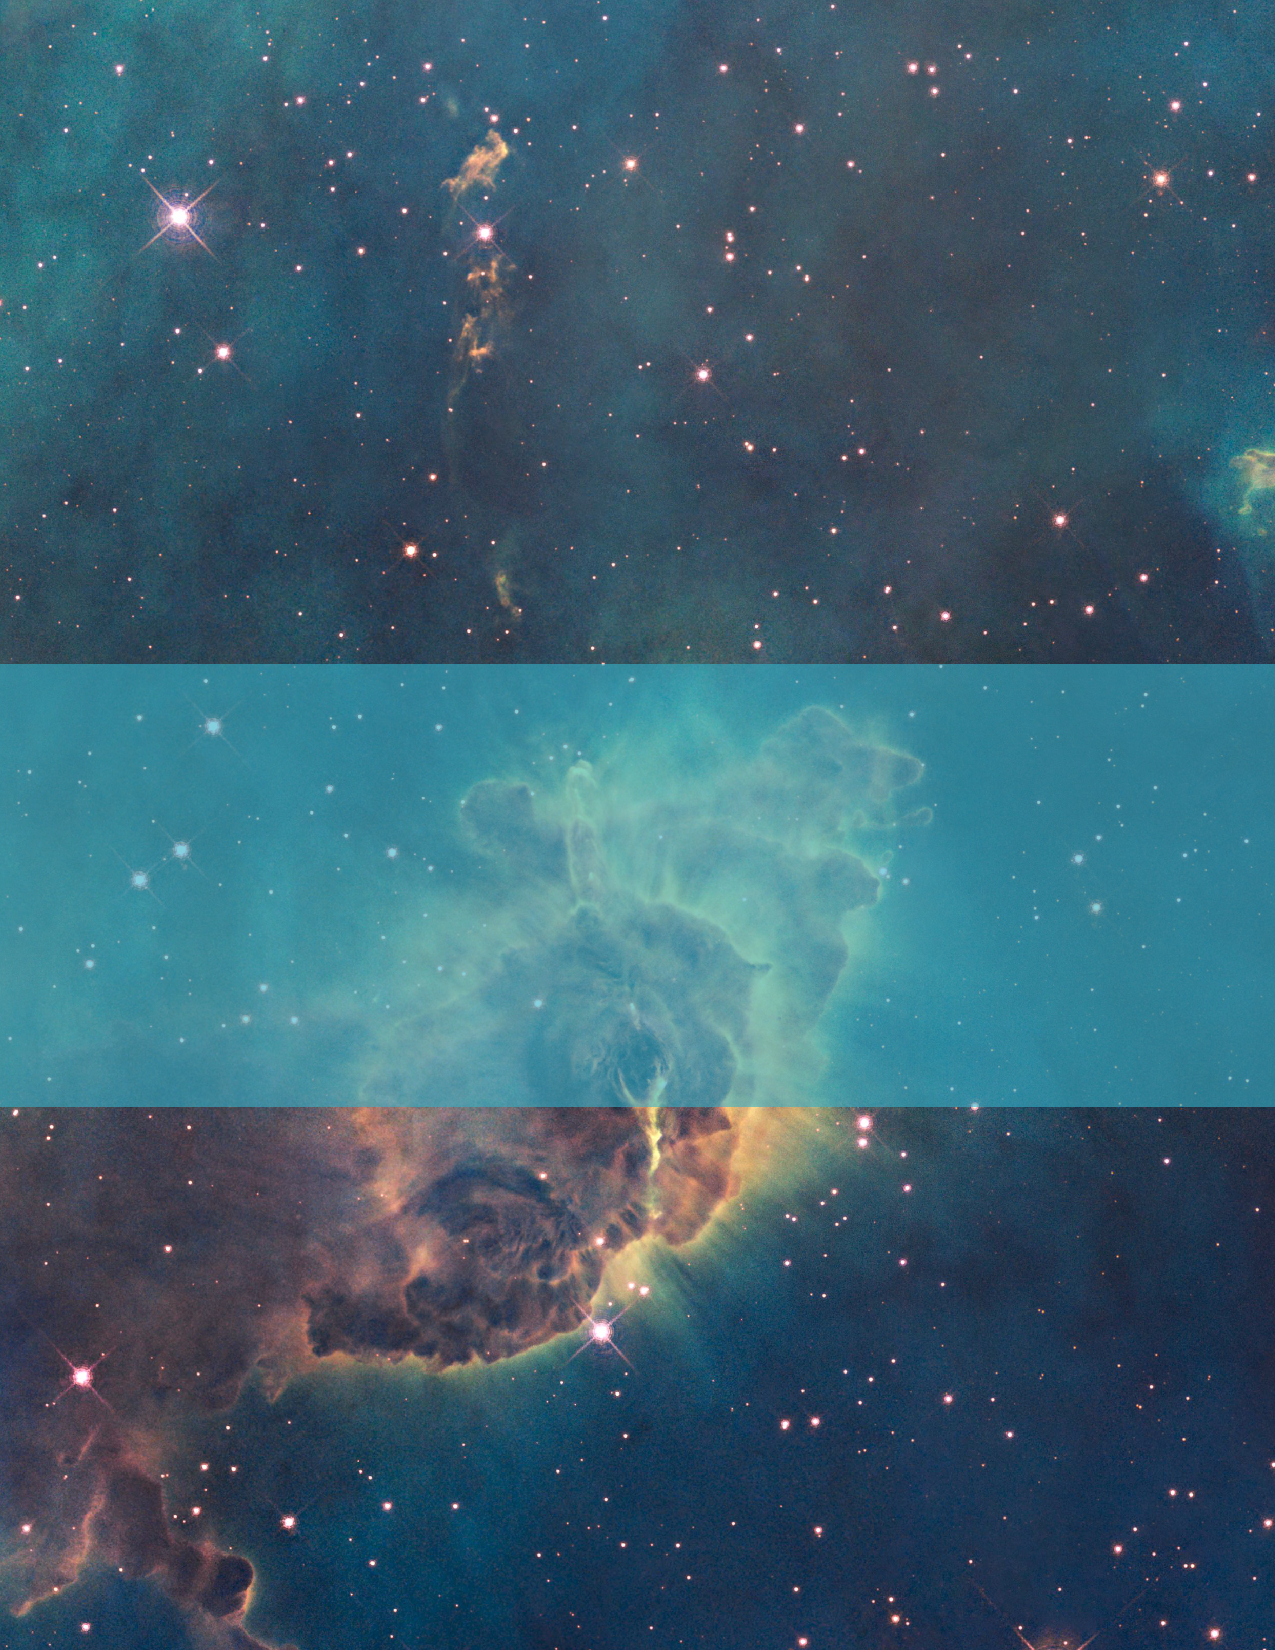
\includegraphics[scale=1.25]{Figures/esahubble}}} % Image background
\centering
\vspace*{5cm}
\par\normalfont\fontsize{35}{35}\sffamily\selectfont
\textbf{Εισαγωγή στην Αστροφυσική}\\
{\LARGE Σάββας Χανλαρίδης}\par % Book title
\vspace*{1cm}
{\Huge Σημειώσεις Μαθήματος}\par % Author name
\endgroup






    % \newcommand{\HRule}{\rule{\linewidth}{0.5mm}}
    % \center
    % % \textsl{\Huge Όνομα Σχολής}\\[0.5cm] 
    % % \textsl{\Large Όνομα Τμήματος}\\[2cm] 
    % \makeatletter
    % \HRule \\[0.6cm]
    % { \huge \bfseries \@title}\\[0.3cm] 
    % \HRule \\[2cm]
    % \large
    % \vspace{5cm}
    % \center 
    % 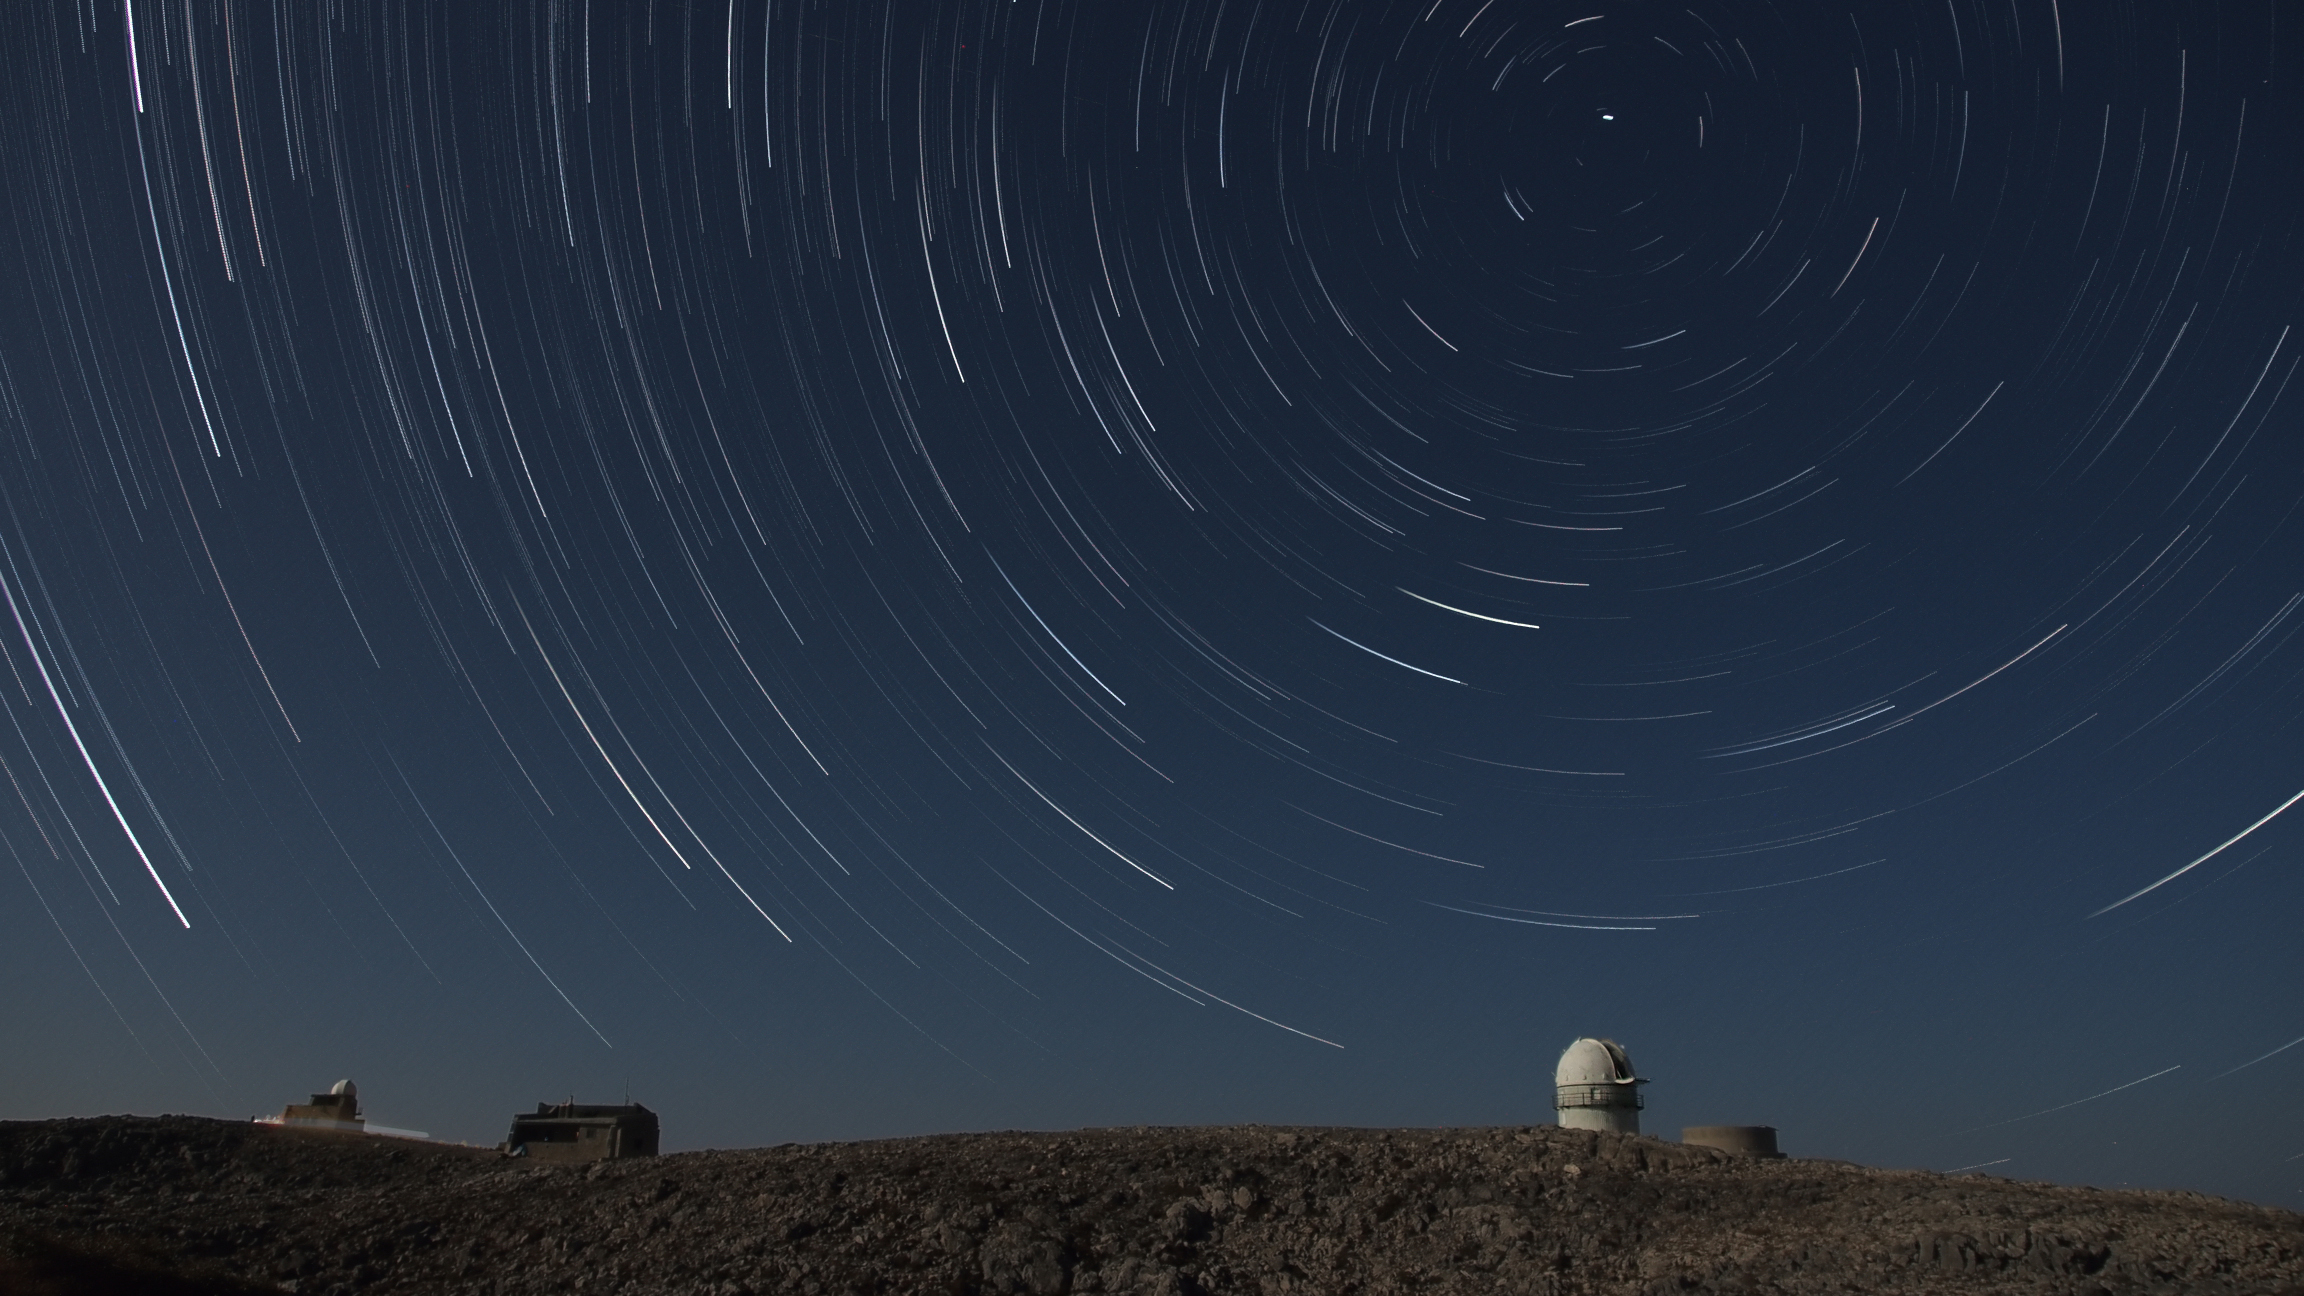
\includegraphics[width=\linewidth]{title/skinakas_star_trails.jpg}
    
   
    % \begin{minipage}{0.45\textwidth}
    % 	\begin{flushleft}
    %         \emph{Συγγραφέας:}\\
    %         \@author \\
    %     \end{flushleft}
    % \end{minipage}
    % ~
    % \begin{minipage}{0.45\textwidth}
    % 	\begin{flushright}
    %         \emph{Υπεύθυνος Καθηγητής:} \\
    %         \textup{Όνομα Καθηγητή}
    %     \end{flushright}
    % \end{minipage}\\[3cm]
    
    % \makeatother
    
    % {\large Η εργασία κατατέθηκε για το μάθημα:}\\[0.2cm]
    % {\Large \emph{Όνομα Μαθήματος}}\\[1cm]
    % {\large \today}\\[2cm]
    % \vfill 
    
\end{titlepage}